\documentclass{acm_proc_article-sp}

\hyphenation{op-tical net-works semi-conduc-tor}

\usepackage{xcolor,graphicx}
\usepackage{verbatim} 
\begin{document}
%
% paper title
% can use linebreaks \\ within to get better formatting as desired
\title{PBJ: A Gnutella Inspired File Sharing System }

% author names and affiliations
% use a multiple column layout for up to three different
% affiliations
\numberofauthors{3}
\author{
\alignauthor
Camden Clements\\
       \affaddr{School of Computing}\\
       \affaddr{Clemson University}\\
       \affaddr{Clemson, SC 29632}\\
       \email{camdenc@gmail.com}
\alignauthor
Adam Hodges\\
       \affaddr{School of Computing}\\
       \affaddr{Clemson University}\\
       \affaddr{Clemson, SC 29632}\\
       \email{hodges8@clemson.edu}
\alignauthor
Zach Welch\\
       \affaddr{School of Computing}\\
       \affaddr{Clemson University}\\
       \affaddr{Clemson, SC 29632}\\
       \email{zwelch@clemson.edu}
}
% conference papers do not typically use \thanks and this command
% is locked out in conference mode. If really needed, such as for
% the acknowledgment of grants, issue a \IEEEoverridecommandlockouts
% after \documentclass

% for over three affiliations, or if they all won't fit within the width
% of the page, use this alternative format:
% 
%\author{\IEEEauthorblockN{Michael Shell\IEEEauthorrefmark{1},
%Homer Simpson\IEEEauthorrefmark{2},
%James Kirk\IEEEauthorrefmark{3}, 
%Montgomery Scott\IEEEauthorrefmark{3} and
%Eldon Tyrell\IEEEauthorrefmark{4}}
%\IEEEauthorblockA{\IEEEauthorrefmark{1}School of Electrical and Computer Engineering\\
%Georgia Institute of Technology,
%Atlanta, Georgia 30332--0250\\ Email: see http://www.michaelshell.org/contact.html}
%\IEEEauthorblockA{\IEEEauthorrefmark{2}Twentieth Century Fox, Springfield, USA\\
%Email: homer@thesimpsons.com}
%\IEEEauthorblockA{\IEEEauthorrefmark{3}Starfleet Academy, San Francisco, California 96678-2391\\
%Telephone: (800) 555--1212, Fax: (888) 555--1212}
%\IEEEauthorblockA{\IEEEauthorrefmark{4}Tyrell Inc., 123 Replicant Street, Los Angeles, California 90210--4321}}

% make the title area
\maketitle


\begin{abstract}
\boldmath
A common basis of differentiating peer to peer (P2P) file sharing applications is by their degree of reliance on a central server.  Some applications, like Napster, rely completely on a central server for organizing users and searching for files.  This kind of structure simplifies system organization and ensures constant time searching.  It also places the burden of the entire system on the server and server failure leads to a total loss of functionality.  Other applications, like gnutella, have no central node, instead connecting users together and passing search requests between users.  This removes the chance of system failure from loss of a single entity, but complicates the network and makes searching less efficient.    

PBJ (Please Be Jenerous) is a file sharing application designed to marry the positive aspects of the centralized and decentralized paradigms.  PBJ users are connected to each other to form a network of users, and requests are passed among them.  To connect users to the system, PBJ uses a central gateway as a simple, powerful way to control the way the network is built to optimize the network. The PBJ gateway allows for increased network stability and efficiency, and if the gateway should go down, existing users can function without it.

\begin{comment}{
 PBJ is based on many of the same principles of the gnutella file sharing application.  Rather than route search requests through some central entity like Napster, PBJ creates a network of connected users.  Search requests are broadcast between users and files are downloaded directly between them.  This paper details the algorithms behind PBJ, the specifics of its implementation, and a comparison of PBJ to other popular file sharing systems.  Future improvements to PBJ are also discussed.   
\end{comment}
\end{abstract}
% IEEEtran.cls defaults to using nonbold math in the Abstract.
% This preserves the distinction between vectors and scalars. However,
% if the conference you are submitting to favors bold math in the abstract,
% then you can use LaTeX's standard command \boldmath at the very start
% of the abstract to achieve this. Many IEEE journals/conferences frown on
% math in the abstract anyway.

% no keywords




% For peer review papers, you can put extra information on the cover
% page as needed:
% \ifCLASSOPTIONpeerreview
% \begin{center} \bfseries EDICS Category: 3-BBND \end{center}
% \fi
%
% For peerreview papers, this IEEEtran command inserts a page break and
% creates the second title. It will be ignored for other modes.




\section{Introduction}

Peer to peer (P2P) file sharing applications are some of the most well known and ubiquitous distributed systems today. These applications allow users of their system to share and download files between each other (usually) free of charge.  In the last fifteen years, file sharing has gone from virtually nonexistent to one of the largest sources of Internet traffic ~\cite{study}.  P2P system structure can vary wildly from highly centralized, in which a single server handles all requests, to highly decentralized, where there are no central elements and the user client programs work together to find results. Beyond basic topology, there are a host of design trade offs.
We were also interested in creating a system that would not be considered liable if illegal content were shared on it. This has been a problem for file sharing applications in the past, particularly Napster. PBJ is a distributed file system that has been designed to be stable, reliable, and able to adapt to changing needs of its users. Due to these design goals, we decided to loosely base the design of PBJ on gnutella, a highly distributed file sharing application. While our overall design is gnutella based, we looked at a range of famous file sharing systems, and several of them influenced our decision making during the design process. 

\section{Related Work}
\subsection{Napster}
A defining characteristic of a P2P file sharing application is the kind of network topology it employs.  Napster, one of the first file sharing networks, was a highly centralized system.  All  online Napster users connected to a central server.  Each user would have a folder designated for sharing audio files (only mp3s were transferred on Napster).  This central server would handle a user request by searching for related files in the share folders of other users.  The central server would then report a list of relevant files and their locations that the user could choose to download.  Any files the requesting user chose to download would directly connect with the associated machine for actual file transfer. Because a given node has only to contact the central server, lookup in Napster can be done in constant time. ~\cite{superpeer}

The ability to search for and download music free of charge was very popular and the Napster user base was very large.  It also happened that a large percentage of the downloads on Napster constituted copyright infringement, since users were distributing music without the creator�s consent. From a legal standpoint, the flaw in Napster�s design was that all of the files on the system were indexed on the central server, including files that broke copyright.  This meant that legally, Napster knew about and facilitated copyright infringement.  In 2001, when the inevitable flood of copyright infringement lawsuits were filed against Napster, a court order shut down the central server.  Because it is a central server, the network ceases to exist when it is taken down. File sharing applications developed after Napster�s shut down attempted to avoid legal liability by making their applications less centralized and by not having their computers keep track of individual files.  Napster exists today as a subscription based service ~\cite{napster}
\begin{comment}
  \subsection{BitTorrent}
 With the dismantling of Napster, file sharing applications started to become more complex and decentralized. Most file sharing today involves the BitTorrent protocol ~\cite{bit}.  BitTorrent differs from other file sharing systems in that it downloads file segments from multiple sources instead of a single file transfer between two users.  BitTorrent works by having a user obtain a torrent file (usually by downloading it from a website).  The local BitTorrent client interprets the contents of the torrent file and connects with a tracker, a server with information about how to find the file. 
 The tracker finds seeders, other BitTorrent clients, with a local copy of the file to be transferred. The file also identifies the swarm, a set of clients with a portion of the file, usually in the process of downloading it themselves.  The searching client downloads from these sources simultaneously to build the desired file.  BitTorrent is especially useful for downloading popular files, since there will be a large pool of seeders and a large swarm.  While BitTorrent is clearly more distributed than Napster, since there are multiple central servers instead of a single large server for the entire application.  However, if the tracker(s) in a torrent file are taken down, there is no way that torrent file can be used to obtain the actual file.     
 \end{comment}

 
   \subsection{Gnutella}
Gnutella (a portmanteau of GNU, the free software project, and Nutella, the chocolate and hazelnut spread) is a decentralized network of interconnected users running a gnutella client called a node.  Search requests are broadcast to all of the searching node�s neighbor clients (which gnutella terms �peers�), which in turn broadcast the request to all of their peers as well ~\cite{lookup}. Lookup in gnutella is $O(log n)$ where $n$ is the number of peers in the system.~\cite{super peer} This goes on until the file is found or the request goes a specified number of peer hops without finding a file (much like the time to live field in an IP packet). A list of the files that match the search are displayed to the user, who then chooses the file to download. The searching node connects directly to the node with the desired file for file transfer. This hop based searching algorithm does allow for the possibility that a search request may fail to return a file in the network, especially as the network gets larger and larger.  Later versions of gnutella�s network introduced the concept of ultra nodes and ultra peers ~\cite{evo}. Each ultra node is connected to a network of regular nodes as well as a large number of other ultra nodes, each having its own network of nodes, making gnutella a network of networks.  The reason for this change is that it allows many more nodes to be reached from any one node in a smaller number of hops, making searching more efficient and the system more scalable.    Nodes keep track of the other nodes they have previously connected with and attempt to reconnect to the network through these nodes.  When connecting for the first time, these nodes must attempt to connect a set of nodes guaranteed to be in the gnutella network.  This means that despite the highly decentralized nature of gnutella, a few centralized elements remain to facilitate the bootstrapping process.  Unlike Napster, which kept information about files on company machines, gnutella does not keep track of the files transferred on their system.  This means that they are not liable if copyright infringement occurs on their system.         

\section{Methodology}
PBJ takes the key qualities of gnutella and uses them only as a starting point, rather than implementing a version of the actual gnutella protocol. Lessons learned from looking at applications like Napster and BitTorrent also played a role in the design of PBJ.  PBJ functions like gnutella in that it creates a network of connected user nodes.  However, it also borrows an important idea from Napster (though slightly altered).  PBJ has a central server running called the gateway.  While Napster kept track of files stored on the system, the gateway keeps track of the nodes in the system and controls the building of the network.  The gateway allows for easy handling of stabilizing the network with nodes being added and removed regularly from the system.  There are three things the PBJ network is designed to handle : building the network, searching the network, and handling node disconnects.  \subsection{Building the Network}
 LIke gnutella, PBJ contains a network of ultra nodes. Each of these ultra nodes has a set of nodes that form an ultra node�s sub network. Ultra nodes in PBJ are given a unique ID starting at 0 and increasing by one each time a new ultra node is added to the network. An ultra node�s ID is assigned in the gateway when it is added to the network. This unique ID is a vital element to building the network. 
 
 \begin{figure}[tbh]
\centering
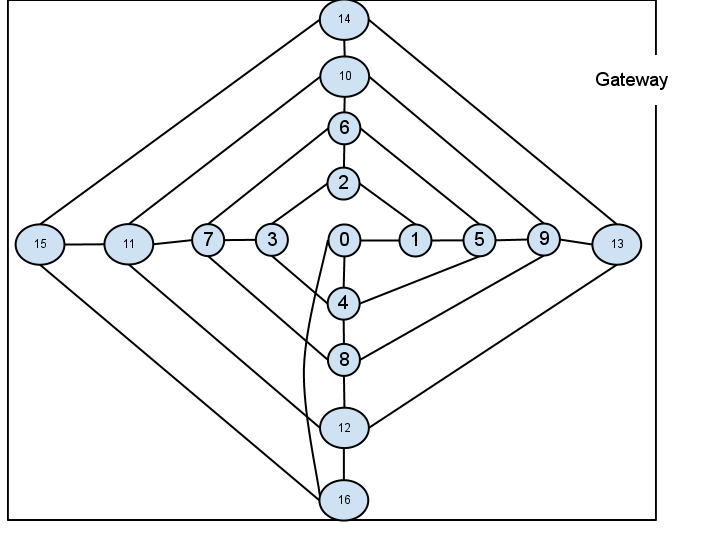
\includegraphics[width=0.5\textwidth]{362prez}
\caption{PBJ Network of Ultra Peers}
\end{figure}
The basic algorithm for connecting ultra nodes in the network builds an outward spiral of ultra peers.  While this alone would be wildly inefficient in terms of searching and stability, new ultra nodes also connect to ultra nodes deeper within the spiral.  This allows search requests to quickly move between otherwise distant ultra nodes. More specifically, the first ultra node created will be given an ID of 0, the second an ID of 1, etc.  When an ultra node is created with ID Y, it will attempt to connect to all nodes $X, 0 < X < Y$, where $\log_2 (|Y - X|) = Z , Z$ being an even integer.  So for example, node 16 would connect with node 15 $(16 - 15 = 1 = 2^0)$, node 12 $(16 - 12 = 4 = 2^2)$, and node 0 $(16 - 0 = 16 = 2^4)$.  

A clear benefit of this structure is that the PBJ network has a high level of redundancy in the connections.  This means that the nodes are connected in such a way that it is easy for search requests to reach most, if not all, of the nodes on the network in a few hops.  Currently, the process of actually adding ultra peers to the network and telling them which other ultra peers to connect to is handled through the gateway. The main job of the gateway is to make decisions about how to add a new user node to the network. The gateway keeps track of the status of all the ultrapeers currently in the system.  When a new node tries to join the system, the gateway makes several decisions based on the current status of the PBJ network.  First, the gateway decides if the new node will become an ultra node.  If so, it will give the new ultra node a list of other ultra nodes to connect to.  If the new node is not an ultra node, the gateway will provide information on the appropriate ultra peer sub network to join. These decisions by the gateway essentially dictate how the network is built. We devised two separate algorithms for building the network; the one we actually implemented is described here and the other is detailed in the section �Future Work�.  As implemented, the first node to enter the network becomes ultra node 0.  If, for example, there are three nodes per ultra node, the next three nodes to connect would become node 0�s sub network.  The fifth node to join the network would become ultra node 1 and would connect to ultra node 0. In this scheme of building the network, each ultra node�s sub network is filled before the next ultra node is created.  This algorithm ensures that the graph has the smallest number of ultra nodes possible in a system and all but potentially the last ultra node have filled sub networks.

\subsection{Searching the Network}

The PBJ client allows a share path to be passed as a command line argument. The default share directory is a subdirectory named �share�. All files and sub directories in the user�s share directory will be available to the network for other nodes to download.  When a user wants to search, they enter a keyword and submit a search request.  The search request will be sent to the searching node�s ultra node (unless the node is itself an ultra node).
\begin{figure}[tbh]
\centering

\includegraphics[width=0.5\textwidth]{search}
\caption{Searching For a File}
\end{figure}

 The ultra node will send the search request to all of the other peers in its sub network before broadcasting it to its connected ultra peers.  Search requests consist of four major parts - the searching node�s address, the keyword, a search id, and the time to live (ttl).  The ttl is initially set to a positive integer.  Each time a search request is passed between ultra peers, the request ttl is decremented.  Notice that ttl only limits the number of hops among ultra peers, passing a request within an ultra node and its sub network has no effect.  If an ultra node receives a search request with a ttl of 0, it will send the request to its sub network and delete the request.  If the keyword is found in any part of a filename, the finding node sends a message to the search node with its IP address and the path of the desired file relative to the share folder.  As these acknowledgement messages come into the search node, it displays to the user a list of all the files found on the network.  The user can then choose one or more of the files to download.  The searching node directly connects to the node with the selected file and downloads it. 
 
 The search ID was added as part of the search request as an attempt to significantly lessen the search request traffic on the network.  The structure of the PBJ network means there are many different paths between any two ultra nodes.  While this is very useful in keeping the network stable and allowing search requests to quickly reach a large number of files, it also means that the same ultra node will receive and process a request multiple times, sending the message out to all of its ultra peers, who have already received the request.  This type of network behavior is extremely inefficient.  PBJ attempts to fix this problem in part by having a unique pair of values in each search request.  One of these values is the IP address of the requester and the other is a search ID that is local to each node and represents the number of requests previously sent out by that node. Together, this (address, search ID) pair make a unique request identifier. Each node keeps track of the last several request ID pairs received and if the request ID pair of a newly received search request matches one in the list, that request is ignored.  This scheme vastly cuts down the amount of redundant request traffic and makes the system more efficient as a whole.     
\subsection{Disconnecting from the Network}
An area of contention during development of PBJ was how to correctly handle ultra peer disconnection.  Various solutions were proposed, including updating the gateway, electing a node from the sub network to be a new ultra node, and the Ostrich approach (ignoring it).  We eventually decided to implement a system of having the gateway check on existing ultra nodes.  Upon receiving a request to add a new node to the network, the gateway pings every ultra node in the network. If one or more does not respond, the gateway marks those as missing, and inserts ultra nodes into these positions until they are all filled. The point here is to ensure that important connections in the network are rebuilt before attempting to refill the sub networks of ultra nodes. In addition, ultra nodes will occasionally ping their ultra peers and sub network.  If an ultra node does not get a response from an ultra peer, it removes it from the list of connected ultra peers.  If an ultra peer cannot connect to a peer in its sub network, it removes that peer from its list and notifies the gateway that a spot has opened up in its sub network.  If a node in a sub network cannot reach its ultra peer, it re enters the network through the gateway.  This ensures that all lost nodes will be replaced as new ones are added to the system, and that the network will not become fractured with high node turnover.  

\section{Results}
All of the PBJ network communication is facilitated through the use of the Flask python module. Flask ~\cite{flask} is a web microframework that is designed to simplify the development of Python web applications. HTTP was chosen as a protocol over TCP due to its reliability, simplicity, and flexibility. Flask trivializes the implementation of custom HTTP responses. Every node, as well as the gateway, is running an instance of a Flask server. The server is configured to run on port 5000 as a default, but this could be easily changed.
Flask was not available as an installed Python module on the lab machines that we were planning on using for our testing, and we did not have administrative privileges to install it, so we needed a way in which we could install and use Flask on every lab machine without modifying any system files. The solution was to use virtualenv ~\cite{virtual}, which is a tool used to create virtual Python environments. A virtual Python environment can be created in a users home folder on a system using virtualenv, and then that user has permission to modify that environment however they wish. In this way, we were able to deploy a Python environment with the Flask module and its dependencies installed on every lab machine.

A concern of ours when laying out the specification of how nodes would communicate was the case in which a node would have to communicate across a firewall. Firewalls add a great deal of complexity when designing a distributed system that is intended to be accessed by a large number of computers under diverse network constraints. Our ultimate decision was that since our project is academic in nature and limited in resources, we were going to ignore the cases in which communication over port 5000 is unavailable to a node.

\subsection{Test Plan}
In order to claim that we have designed a stable and scalable system with confidence, we needed to design a solid testing plan. In the design phase of our project, we thoroughly discussed the use of Condor, a HTC application that can deploy processes to a large number of computers, to test our network stability and search algorithms for large numbers of nodes. Unfortunately, the computers on Clemson�s Condor network are equipped with Windows Firewall, which blocks the access of ports that have not been explicitly granted permission. As previously discussed, we will be ignoring the cases in which our nodes are behind firewalls, so this test strategy was inadequate. Instead, we devised a test strategy in which we wrote a script to connect every available lab machine we had to our network. 

The end result was a test environment in which over 70 search-able nodes with unique files were connected to our network. Although this is a considerable amount of nodes, we found that it was not sufficient to fully test the scaling and performance of our search algorithm. We used this large network of connected nodes primarily to test the functionality and reliability of our system.
The main goals of testing the gateway server was twofold. First, correct network topology was to be maintained when new nodes were added.  This could easily be checked by feeding the gateway a large number of pseudo nodes to verify that the intended topology could be maintained for any size network. Furthermore, an applet was developed to display an image representing the network graph, making it easier to see node to node connections. The second goal of gateway testing was to verify that any dropped node notifications were being handled correctly, which involved updating the network structure for addition of future nodes. This is further discussed later when testing node functions.

Testing node functionality proved to be much more in depth. For this, we developed a series of repeatable test cases that the network should be able to handle. These test cases included: initiating a search as an ultra node, initiating a search as a node, searching from one end of the network to the other, searching from the middle of the network to either end, and downloading a search result. We also monitored the gateway to ensure that the network structure was maintained and rebuilt after all node disconnection scenarios: dropping a node from the beginning, middle, and end of the network, as well as dropping an ultra node from the beginning, middle, and end of the network.
We repeated these test cases after every change we made to ensure that PBJ was stable and working properly.
\section{Analysis}

Our testing demonstrated to us the stability of the network. To a large extent, the main goals of the project were met. A network of connected peers could be created using only a simple centralized gateway, while keeping file searching and downloading independent of such a server. We discovered, however, that there was a large amount of traffic on the network between the pinging of peers and redundant searching, even reduced as it is with the unique request ID. We also feel that an explicit ttl will eventually limit PBJ�s scalability. This section provides an in depth look at our test results and possible improvements future versions of our system could implement to deal with these perceived issues.

\subsection{Future Work}

\subsubsection{Decentralization}
One improvement previously discussed is changing how nodes join the system. The current gateway method functions well, but its centralized nature is hardly ideal for a system whose design so highlights decentralization. Several alternatives have been discussed. The most likely implementation would be to place the burden of network building on the existing ultra nodes.  A node would keep track of its previously connected ultra nodes and attempt to connect to these peers. Depending on its current status, the ultra peer might add the new users or decide to push it towards higher valued ultra peers to attempt placement. Eventually it would either get placed in a sub network or reach the ultra peer with the highest id and become the new highest ultra peer.  If none of the previously connected nodes are currently connected to the network, a range of options could be implemented to ensure the user gets into the network including but not limited to: keeping the gateway as a backup, having ultra nodes at known URLs, placing the burden on the user to find the information.

\subsubsection{Network topology}
Several different specific algorithms for how exactly the network is organized were discussed. The current algorithm, described above, creates a new ultra node and then fills that ultra node�s sub network before creating a new ultra peer. While this algorithm works acceptably, it ignores several observations about PBJ�s network. In PBJ, the number of hops it takes to get from node A to node B is highly dependent on the current number of ultra peers in the system. As a simple example, the optimal number of hops from ultra peers 0 to 63 is 5 hops (0-16-32-48-47-63) if ultra node 64 does not exist and 2 hops (0 -64-63) if ultra node 64 does exist. Indeed, a node whose largest hop was one of the last nodes to be added has the optimal network structure for searching.

 Our algorithm for taking advantage of this trait slightly alters how the network is built by the gateway. The basic idea behind this algorithm is to have an ultra peer back bone in place first with empty sub networks and then fill in the sub networks. When creating a new network, the first eight (eight is half of sixteen) nodes into the system will become the first eight ultra peers. The next nodes to join the system will join these ultra peers� sub networks. When all eight sub networks have been filled, the gateway then add the next nodes as ultra peers in the system until there are thirty-two ultra peers (thirty two is half of sixty four) in the system. This continues so that when the network is full, it grows to half the size of the next even power of two before filling in the ultra peers. This ensures that the majority of the peers are close together but have the ability to move farther because there is an ultra peer structure in place to facilitate such movement.  Another potential improvement would be to choose ultra peers based on network quality. Ultra peers have to handle the vast majority of the network traffic. It then makes sense that the machines with the strongest network connection should be ultra peers. This would help stabilize the network and improve quality.

\subsubsection{Searching}
We also feel the search algorithm could be improved or a new algorithm implemented. Going forward, it seems that the ttl is the main issue to be addressed. Its purpose is to limit system traffic, but if the network becomes large enough, it is possible searches from a certain node will never reach other machines far enough away in the network. Though additional testing would be necessary, we would need to see the effects of larger ttl values on system traffic. It may make sense to remove the ttl all together and count on the unique ID checking to limit redundant network traffic. We have also discussed tiers of ttl values corresponding to the size of the hop to be taken. This algorithm is still early in development and would need more research.  

\subsubsection{Stabilization}
Handling node failure was a tough challenge in early development. As convenient and stabilizing as our node ping method for detecting disconnected nodes is to the network, it leads to a lot of network traffic. Currently, nodes ping each other every few seconds. It might make sense to have nodes ping only right before sending a search request, or to implement some kind of TCP style application level three way hand shake. In addition, it might make sense for ultra nodes to contact the gateway when they have lost contact with an ultra peer, rather than having the gateway ping all ultra nodes in the network.    

\subsubsection{User experience}
Simple things such as an improved GUI and security/privacy features could also be added to make the system more user friendly. Another concern we have is attempting to mitigate is leeching, the practice where by users of a file sharing network do not share any files to be downloaded but still use the network to get files.

\section{Conclusion}

PBJ is a decentralized file sharing system whose highly connected nodes, search algorithm, and intelligent node loss handling make the ground work for a stable and reliable application. PBJ is heavily influenced by existing file sharing services gnutella and to a much lesser extent Napster. PBJ users connect to the system through a dedicated gateway, either becoming ultra nodes connected to other ultra nodes or part of an ultra node�s sub network. Searching the network is done by keyword comparison to filenames, and search requests are broadcast between ultra peers.

 Results are displayed to the user to choose a result to download. The gateway and the nodes themselves periodically ping their connections. If an ultra peer does not respond to a ping, it is removed from the ultra node�s active connections.  If a sub network node�s ultra node does not respond, the node will exit the network and attempt to reconnect through the gateway. Every time the gateway attempts add a node, it first checks that existing ultra peers are connected.  If one has gone down, the node to be added is added in that ultra peer�s place. PBJ uses Flask for network communication.

Thorough unit testing of both gateway server and node application functions proved the functionality of the PBJ network. It also let us see what areas of the sharing system need the most attention in order to improve performance. Network scalability and stability were seen to be correct and fully functional as intended.
Based on this testing, however, we have a number of future improvements to PBJ.  These improvements would increase the network�s stability, decrease redundant traffic, and reach a larger percentage of the network.


% conference papers do not normally have an appendix


% use section* for acknowledgement
\section*{Acknowledgment}


The authors would like to thank Dr. Goasguen for his help and advice, the Clemson University Systems staff for quickly responding to the various technical problems and hurdles faced in setting up machines for testing, and Dunkin Donuts for making their delicious coffee the authors used in the majority of this project.




% trigger a \newpage just before the given reference
% number - used to balance the columns on the last page
% adjust value as needed - may need to be readjusted if
% the document is modified later
%\IEEEtriggeratref{8}
% The "triggered" command can be changed if desired:
%\IEEEtriggercmd{\enlargethispage{-5in}}

% references section

% can use a bibliography generated by BibTeX as a .bbl file
% BibTeX documentation can be easily obtained at:
% http://www.ctan.org/tex-archive/biblio/bibtex/contrib/doc/
% The IEEEtran BibTeX style support page is at:
% http://www.michaelshell.org/tex/ieeetran/bibtex/
%\bibliographystyle{IEEEtran}
% argument is your BibTeX string definitions and bibliography database(s)
%\bibliography{IEEEabrv,../bib/paper}
%
% <OR> manually copy in the resultant .bbl file
% set second argument of \begin to the number of references
% (used to reserve space for the reference number labels box)
\begin{thebibliography}{99}

\bibitem{evo}
Amir H. Rasti, Daniel Stutzach, Reza Rejaie, "On the Long term Evolution of the Two Tier Gnutella Overlay", in \emph{INFOCOM Proceedings}, Barcelona, Spain, 2006, pp 1 - 6
\bibitem{napster}
Napster Website: http://www.napster.com
\bibitem{bit}
BitTorrent Website: http://www.bittorrent.com/
\bibitem{compare}
Dimitrios Tsoumakos and Nick Roussopoulos. (2011, 11, 20) "A comparison of Peer to Peer Search Methods" [Online]. Available : Google Scholar
\bibitem{flask}
Flask Website : http://flask.pocoo.org/
\bibitem{virtual}
Virtualenv Website : http://www.virtualenv.org/en/latest/index.html
\bibitem{lookup}
Hari Balakrishnan et al, "Looking Up Data in P2P Systems". \emph{Communications of the ACM}, vol 46, No 3,  February, 2003.
\bibitem{study}
Hendrik Schuleze and Klaus Mochalski. "Internet Study 2008/2009". Ipoque Leipzig Germany, 2009
\bibitem{superpeer}
Alper Tugay Misrak et al. "Structured Superpeers: Leveraging Heterogeneity to Provide Constant-Time Lookup" . \emph{WIAPP 2003 Proceedings}
\bibitem{saroiu}
S. Saroiu, P. Gummadi, S. D. Gribble,  \emph{A Measurement Study of Peer-to-Peer File Sharing Systems}, 
University of Washington Technical Report UW-CSE-01-06-02, July 2001.
\bibitem{adar}
Eytan Adar , Bernardo A. Huberman. " Free Riding on Gnutella". 2000

\end{thebibliography}




% that's all folks
\end{document}


